\chapter{Design Evaluation}
\label{cha:measurements}
For measuring the effect of different designs on the simulation's performance, an example network was implemented using a monolithic and a modular design.
These implementations represent examples of the designs discussed in chapter \ref{cha:design}.


\section{Simulated Example Network}
\label{sec:measurements_network}
The example network simulates a message queue with dispatching of different types of transmitted data (configuration, event, historical).
The different types of data are processed by different parts within the network.
This network includes parts for data generation and data processing.
Such an exemplary network was chosen, in view of multiple similar practical applications.
An overview of the simulated network is shown in Figure \ref{fig:design_test_network}.

\begin{figure}
    \centering
    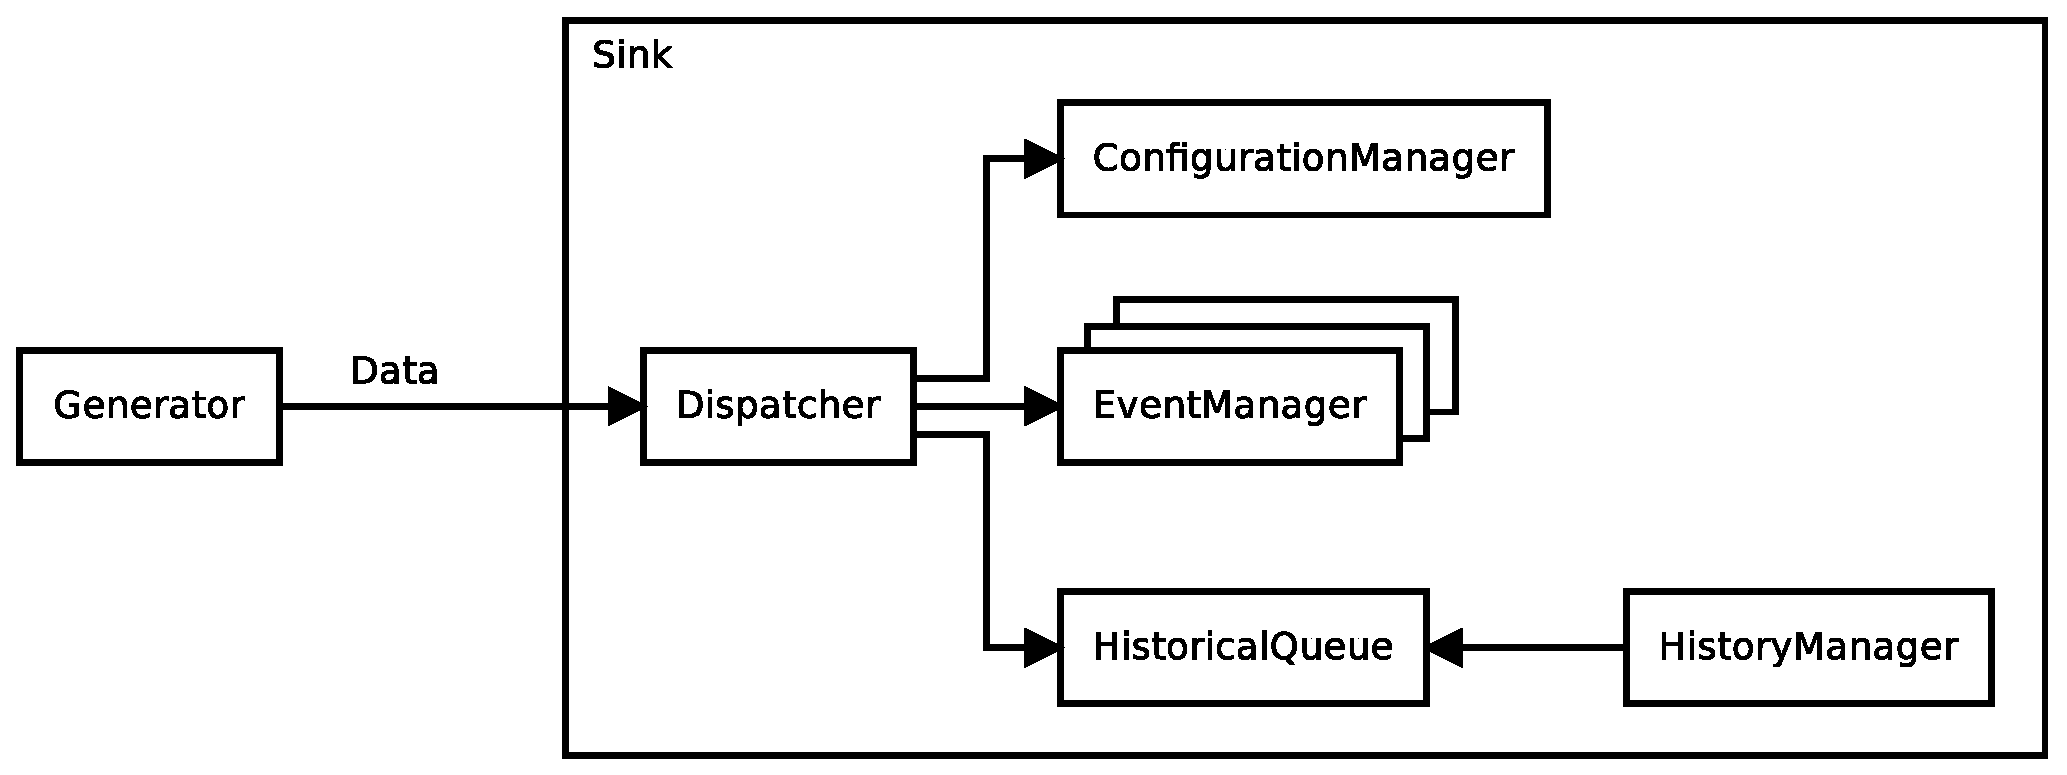
\includegraphics[width=0.9\linewidth]{design_test_network.eps}
    \caption{Example network including \emph{Generator}, \emph{Sink}, \emph{HistoricalQueue} and the data processing modles \emph{ConfigurationManager}, \emph{EventManager}, and \emph{HistoryManager}.}
    \label{fig:design_test_network}
\end{figure}

The \emph{Generator} generates cyclic data which is transmitted via messages to the sink module.
The generated data includes a field of 64 bytes and an enumeration describing the type of data.

These messages are transmitted to a sink, which is described via the interface module \emph{ISink}.
The differently designed modules \emph{ModularSink} and \emph{MonolithicSink} extend the interface and represent the differently tested designs.

The first part within the sink is the \emph{Dispatcher} which accesses the type information of the data and then forwards the packed data to the according managers or the \emph{HistoricalQueue}.
The simulated network provides a variable number of \emph{EventManagers}, all generated events are dispatched to the \emph{EventManagers} sequentially.
The \emph{ConfigurationManager} and the \emph{EventManagers} are simple implementations which executes various calculations on the received data to simulate processing.
Historical data are forwarded to the \emph{HistoricalQueue} which is internally implemented by a std::queue that holds all received data until they are accessed.
The \emph{HistoryManager} accesses the \emph{HistoricalQueue} and processes available data similar to \emph{ConfigurationManager} and \emph{EventManager} by executing dummy calculations.
This access is initiated by the \emph{HistoryManager} itself and provides a configurable polling interval.
\\

The functionality of dispatching and processing the data is, as shown in Figure \ref{fig:design_test_network}, included in the sink and is implemented twice with different designs.

The assumption of existing implementations for the \emph{Dispatcher}, \emph{HistoricalQueue}, \emph{ConfigurationManager}, \emph{EventManager} and \emph{HistoryManager} is made.
This assumption should connect this design test to practical scenarios, where existing code cannot be changed for the simulation.
Therefore, implementing the \emph{MonolithicSink} consists of instantiating and connecting the different parts within a single simple module.
Received messages will be analyzed and the enclosed data is forwarded to the according instances.
The polling is done by the \emph{ConfigurationManager} using \emph{self-messages} sent in an configurable interval.

Implementing the \emph{ModularSink} requires the implementation of wrapper modules for every single part which should be represented by a separate module.
These wrapper extract the transmitted data of received messages and forward them to the enclosed parts.
Calls from within the enclosed parts are handled by methods of the wrappers, which are passed via function pointers (functional objects).
Within those methods relevant messages are created and sent via the correct output gates.
The internal structure of the \emph{ModularSink} is shown in Figure \ref{fig:ModularSink}.
Within the \emph{ModularSink} arrays of gates, connections and instances of \emph{EventWrappers} are used for realizing a variable number of \emph{EventManagers}.

\begin{figure}
    \centering
    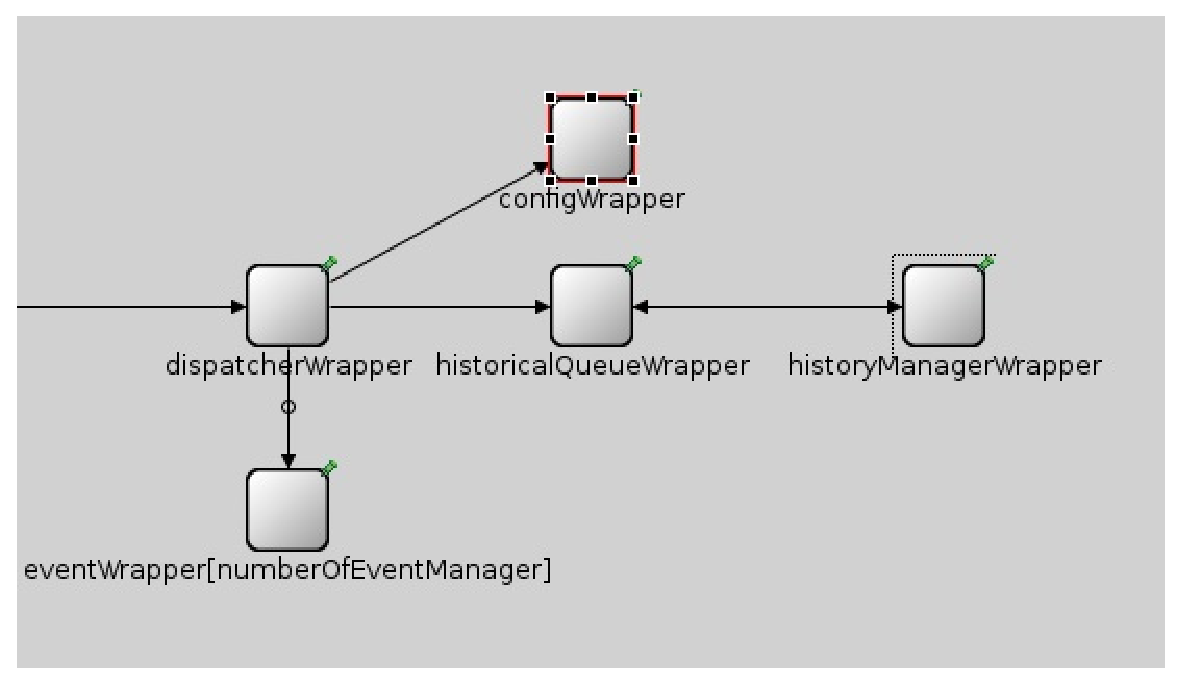
\includegraphics[width=0.9\linewidth]{images/ModularSink}
    \caption{Structure of \emph{ModularSink} showing the implemented wrapper modules and their connections.}
    \label{fig:ModularSink}
\end{figure}

The simulated network consists of the \emph{Generator} instance and an instance specializing \emph{ISink} the underlying module and therefore the tested design is configured via a variable type.
The resulting network for data generation is shown in Figure \ref{fig:omnet_example_network}.

\begin{figure}
    \centering
    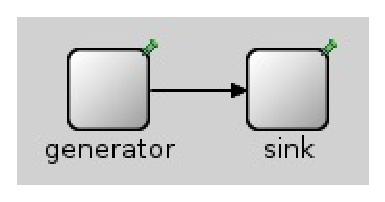
\includegraphics[width=0.3\linewidth]{images/omnet_example_network}
    \caption{Simulated example network showing the \emph{Generator} instance and its connection to the instance of the sink module derived from \emph{ISink}.}
    \label{fig:omnet_example_network}
\end{figure}

\section{Measurement Methods}
\label{sec:measurements_methods}
For measuring the performance of the different designs, three measurement methods were implemented.
The implementation of different methods was done for preventing false assumptions based on the result of a single test.
These methods were implemented via different scripts for automated execution and designed dynamically allowing for the analysis of various simulations and also either sequential or parallel simulation.

\subsection{Runtime Measurement}
\label{sec:measurements_methods_runtime}
The performance of the simulated design can be analyzed by defining a fixed simulation time limit (\emph{sim-time-limit}).
The usage of the default (non real-time) scheduler results in a simulation which executes as fast as possible for the required number of events for reaching the simulation time limit.
The required execution time for this simulation represents the performance of the simulation.

Analyzing a parallel simulation using this method does not require special attention, except the handling of multiple resulting runtime values.

\subsection{Processed event count}
\label{sec:measurements_methods_event}
By defining a fixed execution time limit (\emph{cpu-time-limit}) and using the default scheduler, the simulation will run for a fixed time.
The number of processed events within this fixed time represents the performance of the simulation.

The simulation of different designs results in contrasting event counts due to the varying number of messages using other designs with more modules and therefore more communication.
For a comparison of the performance, the created number within a fixed processing time a correction factor must be considered.
This factor describes the ratio of created events using the different designs.
This ratio can be measured by using the configuration of the previous method \ref{sec:measurements_methods_runtime} and analyzing the number of created events.

Analyzing a parallel simulation and comparing the performance to a sequential simulation requires further attention to the number of created events.
An additional correction factor is necessary due to the varying number of sent synchronization messages.
Because of this additional correction factor and the increasing uncertainty coming with it, this measurement method was not used for parallel simulation.

\subsection{Real-time Behavior}
\label{sec:measurements_methods_realtime}
Using the built-in real time scheduler \emph{cRealTimeScheduler} the simulation will try to execute the simulation matching the real time.
The performance output (\emph{cmdenv-performance-display}) provides the ratio of simulated seconds per real second.
As described in section \ref{sec:simulation_omnet}, this ratio must not differ too much from one for representing a real-time simulation.
The simulated network provides a configurable interval of data generation by \emph{Generator}.
Using a parameter study (described in section \ref{sec:omnet_running_config}) the interval for data generation by \emph{Generator} can be set to values form a range of intervals.
With attention to the performance ratio of the different iterations, the interval limit, which still allows for real-time simulation, can be determined.

Running an OMNeT++ simulation parallelized demands the definition of a synchronization class implementing the used synchronization algorithm as described in section \ref{sec:parallel_omnet_sync}.
A synchronization class used in OMNeT++ is derived from the base class \emph{cParsimSynchronizer}.
This base class implements a \emph{cScheduler} and during a parallel simulation, it is also used as a scheduler.
To achieve a parallel real-time simulation a custom synchronization class enclosing the behavior of a real-time scheduler must be implemented.
Due to the lack of such a built-in synchronization class the measurement method for testing the real-time behavior was not used for testing the parallel simulation.

\subsection{Result Recording}
The results of the different measurement methods are all extracted from the resulting command line output of the simulation.
The automated test scripts analyze the outputs of the executed simulation after finishing the simulation.
For preventing the delay of the measurements and the simulation by writing the output to a file located on a slow peripheral, the output files are located on a \emph{ramdisk}.
A \emph{ramdisk} represents a filesystem which is located within the \emph{RAM} (Random access memory) and therefore provides the maximum speed for writing and analyzing outputs.

The implemented test network described in \ref{sec:measurements_network} was developed and analyzed on a Lenovo ideapad U530 with 8GB PC3-12800 DDR3 SDRAM 1600 MHz and a 4th Gen Intel® Core™ i7-4500U (1.8 GHz 200 MHz 4MB) running Kubuntu 15.10.
\cite{lenovo_spec}

\section{Sequential Simulation}
\label{sec:measurements_sequential}
Each of the three developed measurement methods was executed multiple times with the example network.
To eliminate a possible dependency of the resulting performance to the simulated range (e.g. period of simulation time), each method was executed with different times.
The runtime and real-time method was executed for multiple values for the simulation time limit and the event method was executed for different cpu time limits.
This variation of simulation time verifies the testing measurements for independence of the simulated time range and provides reference values for determining correction values for the event method \ref{sec:measurements_methods_event}.

By simulating multiple scenarios, three parameter studies (parameter sweeps) were executed for each testing method.

\begin{itemize}
    \item Number of EventManager (default = 1)
    \item Generation interval of \emph{Generator} (default = $100\mu s$)
    \item Polling interval of \emph{HistoryManager} (default = $100\mu s$)
\end{itemize}

During the simulation with different values of a single parameter study the other values are set to the default values.
For the testing scenarios, the simulation time limit for the runtime and real-time method or the cpu time limit for the event method was set to one minute arbitrarily.
In the following section, the measurement result of the evaluation test (sweep of simulation or cpu time) and the results of the test scenarios are shown and analyzed.

\subsection{Runtime}
\label{sec:measurements_sequential_runtime}

The runtime results of the sequential simulations using both designs and given different simulation time limits are displayed in Figure \ref{fig:results_runtime_sim_time}.
The double logarithmic axis shows two linear characteristics for modular and monolithic design.
These nearly parallel linear characteristics show a constant factor between the runtimes using the two different designs.
The average ratio of runtime using the modular design over the runtime using the monolithic design is $3.393$.
\\

%%% runtime over simulation time %%%
\begin{figure}
    \centering
    \pgfplotsset{
        every axis plot/.append style={very thick}
    }
    \begin{tikzpicture}
        \begin{axis}[
        xmode=log,
        ymode=log,
        ylabel={Runtime $[s]$},
        xlabel={Simulation time $[s]$},
        grid=major,
        legend entries={Modular,Monolithic},
        legend style={at={(0.03,0.97)}, anchor=north west}
        ]
        
        \addplot table {../results/lenovo/runtimeResults.Modular.txt};
        \addplot table {../results/lenovo/runtimeResults.Monolithic.txt};
        \end{axis}
    \end{tikzpicture}    
    \caption{Runtime using different designs over different simulation time limits.}
    \label{fig:results_runtime_sim_time}
\end{figure}

The runtime using different designs with a varying number of \emph{EventManagers} is shown in Figure \ref{fig:results_runtime_eventmanager}.
As expected, there is no obvious dependency of the resulting runtime on the number of included \emph{EventManagers}.
Due to the fixed simulation time, the number of created event stays the same.
The only difference introduced by the increasing number of \emph{EventManagers} is the destination of the event type data.
The required time for transporting the messages and processing the data is untouched.
The increasing number affects the memory usage of the simulation, which is not analyzed within this design test.
The offset, visible in Figure \ref{fig:results_runtime_eventmanager}, between the different designs represents the ratio of achieved performance regarding the runtime.
The average of this ratio is $3.342$.
\\

%%% runtime over number of event manager %%%
\begin{figure}
    \centering
    \pgfplotsset{
        every axis plot/.append style={very thick}
    }
    \begin{tikzpicture}
    \begin{axis}[
    xmode=log,
    %ymode=log,
    ylabel={Runtime [s]},
    xlabel={Number of \emph{EventManager}},
    grid=major,
    legend entries={Modular,Monolithic},
    legend style={at={(0.97,0.5)},anchor=east}
    ]
    
    \addplot table {../results/lenovo/time/simtimeEventManagerResults.Modular.txt};
    \addplot table {../results/lenovo/time/simtimeEventManagerResults.Monolithic.txt};
    \end{axis}
    \end{tikzpicture}    
    \caption{Runtime using different designs over variing number of \emph{EventManager}.}
    \label{fig:results_runtime_eventmanager}
\end{figure}

The runtime using different designs with a varying polling interval by the \emph{HistoryManager} is shown in Figure \ref{fig:results_runtime_polling}.
These results are further displayed in a double logarithmic plot for easier recognition of both plots following a potential characteristic, which is visible as linear plots.
As expected the required runtime decreases with increasing polling interval.
This behavior can be explained by the sinking frequency of polling operations and thus a decreasing communication.
The offset between the two plots is shown in Figure \ref{fig:results_runtime_polling}, due to the double logarithmic display, representing the ratio between the runtimes using different designs.
The average ratio of runtime using the modular design over the runtime using the monolithic design is $7.809$.
\\
%%% runtime over polling interval %%%
\begin{figure}
    \centering
    \pgfplotsset{
        every axis plot/.append style={very thick}
    }
    \begin{tikzpicture}
    \begin{axis}[
    xmode=log,
    ymode=log,
    ylabel={Runtime [s]},
    xlabel={Polling interval [ns]},
    grid=major,
    legend entries={Modular,Monolithic},
    legend style={at={(0.97,0.97)}, anchor=north east}
    ]
    
    \addplot table {../results/lenovo/time/simtimePollingResults.Modular.txt};
    \addplot table {../results/lenovo/time/simtimePollingResults.Monolithic.txt};
    \end{axis}
    \end{tikzpicture}    
    \caption{Runtime using different designs over varying polling interval by the \emph{HistoryManager}.}
    \label{fig:results_runtime_polling}
\end{figure}

\newpage

The runtime using different designs with a varying generation interval by the \emph{Generator} is shown in Figure \ref{fig:results_runtime_generation}.
Similar to the previous Figure these results are also shown in a double logarithmic plot showing the potential characteristic of sinking required runtime with increasing generation interval.
Again the noticeable offset between the plots is due to a ratio of resulting runtimes.
The average ratio of runtime using the modular design over the runtime using the monolithic design is $1.588$.
\\

%%% runtime over generation interval %%%
\begin{figure}
    \centering
    \pgfplotsset{
        every axis plot/.append style={very thick}
    }
    \begin{tikzpicture}
    \begin{axis}[
    xmode=log,
    ymode=log,
    ylabel={Runtime [s]},
    xlabel={Generation interval [ns]},
    grid=major,
    legend entries={Modular,Monolithic},
    legend style={at={(0.97,0.97)}, anchor=north east}
    ]
    
    \addplot table {../results/lenovo/time/simtimeGenerationResults.Modular.txt};
    \addplot table {../results/lenovo/time/simtimeGenerationResults.Monolithic.txt};
    \end{axis}
    \end{tikzpicture}    
    \caption{Runtime using different designs over varying generation interval by the \emph{Generator}.}
    \label{fig:results_runtime_generation}
\end{figure}


Analyzing the resulting outputs the ratio of generated messages (events) regarding the different designs can be determined.
The average ratio of number of created events using the modular design over the number of created events using the monolithic design is $2.149$.
This ratio will be used as correction value for the next measurement method analyzing the created events within a fixed cpu time.

\subsection{Created Events}
\label{sec:measurements_sequential_event}

The results of testing the simulations and analyzing the number of created events within a given cpu time are displayed in Figure \ref{fig:results_event_cpu_time}.
Similar to the previous section, a double logarithmic display was used for analyzing the characteristic of the plots.
The courses show potential characteristics and are nearly linear and parallel, which leads to the assumption of a constant ratio between the used designs.
The average ratio of the number of created events using the modular design over the number of created events using the monolithic design is $0.284$.
For comparison to the previous and following test method, the reciprocal value is calculated and equals $3.521$.
\\

%%% event number over cpu time %%%
\begin{figure}
    \centering
    \pgfplotsset{
        every axis plot/.append style={very thick}
    }
    \begin{tikzpicture}
        \begin{axis}[
        xmode=log,
        ymode=log,
        ylabel={Created event},
        xlabel={Cpu time $[s]$},
        grid=major,
        legend entries={Modular,Monolithic},
        legend style={at={(0.03,0.97)}, anchor=north west}
        ]
        
        \addplot table {../results/lenovo/eventResults.Modular.txt};
        \addplot table {../results/lenovo/eventResults.Monolithic.txt};
        \end{axis}
    \end{tikzpicture}    
    \caption{Created events for different designs over different cpu time limits.}
    \label{fig:results_event_cpu_time}
\end{figure}

The number of created events using different designs and a varying number of \emph{EventManagers} is shown in Figure \ref{fig:results_event_eventmanager}.
As expected and similar to the results of the runtime with a varying number of \emph{EventManagers} there is no noticeable dependency of the created events on the number of \emph{EventManagers}.
This presumption is due to the change of number of instantiated \emph{EventManagers}, whereby only the destination of the transmitted events is affected and not the number of events.
Using the double logarithmic scale the ratio between the different designs is visible as offset, which is shown in Figure \ref{fig:results_event_eventmanager}.
This ratio is defined by the number of created events using a modular design over the number of created events using a monolithic design.
The average of this ratio is $0.273$.
In comparison between the previous and following test method the reciprocal value is calculated which equals $3.663$.
\\

%%% events over Event managers %%%
\begin{figure}
    \centering
    \pgfplotsset{
        every axis plot/.append style={very thick}
    }
    \begin{tikzpicture}
    \begin{axis}[
    xmode=log,
    %ymode=log,
    ylabel={Created events},
    xlabel={Number of EventManager},
    grid=major,
    legend entries={Modular,Monolithic},
    legend style={at={(0.97,0.5)},anchor=east}
    ]
    
    \addplot table {../results/lenovo/event/cputimeEventManagerResults.Modular.txt};
    \addplot table {../results/lenovo/event/cputimeEventManagerResults.Monolithic.txt};
    \end{axis}
    \end{tikzpicture}    
    \caption{Created events using different designs over varying number of \emph{EventManager}.}
    \label{fig:results_event_eventmanager}
\end{figure}

The number of created events using different designs and a varying polling interval by the \emph{HistoryManager} is shown in Figure \ref{fig:results_event_polling}.
The expected behavior would be a sinking number of created events with increased polling interval by the \emph{HistoryManager}.
This behavior should be introduced by the decreased frequency of polling messages or self messages for timer implementations and therefore an increased number of created messages.
Analyzing the characteristics shown in \ref{fig:results_event_polling} displays this behavior only using the monolithic design.
Due to this mismatch of both behaviors, no assumption about the dependency is made.
The offset between the plots using different designs is nevertheless indicating a ratio representing the performance difference of the used designs.
This ratio is defined by the number of created events using a modular design in contrast to those using a monolithic design.
For this test the average of this ratio results in $0.170$.
In comparison to the previous and following test method the reciprocal value is calculated and equals $5.882$.
\\

%%% events over polling interval %%%
\begin{figure}
    \centering
    \pgfplotsset{
        every axis plot/.append style={very thick}
    }
    \begin{tikzpicture}
    \begin{axis}[
    xmode=log,
    ymode=log,
    ylabel={Created events},
    xlabel={Polling interval [ns]},
    grid=major,
    legend entries={Modular,Monolithic},
    legend style={at={(0.03,0.5)},anchor=west}
    ]
    
    \addplot table {../results/lenovo/event/cputimePollingResults.Modular.txt};
    \addplot table {../results/lenovo/event/cputimePollingResults.Monolithic.txt};
    \end{axis}
    \end{tikzpicture}    
    \caption{Created events using different designs over varying polling interval by the \emph{HistoryManager}.}
    \label{fig:results_event_polling}
\end{figure}

The number of created events using different designs and a varying generation interval by the \emph{Generator} is shown in Figure \ref{fig:results_event_generation}.
Similar to the polling interval of \emph{HistoryManager} shown in \ref{fig:results_event_polling} number of created events should be sinking with increased generation interval.
In this scenario only the usage of the modular design shows this characteristic and thus no assumption about the dependency is made.
The offset is related to the ratio between the designs and the average ratio is $0.414$.
In comparison to the previous and following test method the reciprocal value is calculated and equals $2.415$.
\\

%%% events over generation interval %%%
\begin{figure}
    \centering
    \pgfplotsset{
        every axis plot/.append style={very thick}
    }
    \begin{tikzpicture}
    \begin{axis}[
    xmode=log,
    ymode=log,
    ylabel={Created events},
    xlabel={Generation interval [ns]},
    grid=major,
    legend entries={Modular,Monolithic},
    legend style={at={(0.97,0.5)},anchor=east}
    ]
    
    \addplot table {../results/lenovo/event/cputimeGenerationResults.Modular.txt};
    \addplot table {../results/lenovo/event/cputimeGenerationResults.Monolithic.txt};
    \end{axis}
    \end{tikzpicture}    
    \caption{Created events using different designs over varying generation interval by the \emph{Generator}.}
    \label{fig:results_event_generation}
\end{figure}

\subsection{Real-time}
\label{sec:measurements_sequential_realtime}

The real-time results of the sequential simulations using both designs and given different simulation time limits are displayed in Figure \ref{fig:results_realtime_sim_time}.
The simulation time limit defines the runtime of a real-time simulation, but does not affect the performance, i.e. the frequency and complexity of calculations.
Therefore as expected the result shows no recognizable dependency of the achievable generation interval to the simulation time.
Although an offset between the different designs is visible.
This offset represents the ratio of achievable generation interval using a modular design in contrast to a monolithic design.
The average of this ratio is $1.717$.\\

% realtime over sim time
\begin{figure}
    \centering
    \pgfplotsset{
        every axis plot/.append style={very thick}
    }
    \begin{tikzpicture}
        \begin{axis}[
        xmode=log,
        ymode=log,
        ylabel={Achievable real time generation interval [ns]},
        xlabel={Simulation time [s]},
        grid=major,
        legend entries={Modular,Monolithic},
        legend style={at={(0.97,0.97)}, anchor=north east}
        ]
        
        \addplot table {../results/lenovo/realTimeResults.Modular.txt};
        \addplot table {../results/lenovo/realTimeResults.Monolithic.txt};
        \end{axis}
    \end{tikzpicture}    
    \caption{Real-time results for different designs over different simulation time limits.}
    \label{fig:results_realtime_sim_time}
\end{figure}

The real-time results for a varying number of \emph{EventManagers} are shown in Figure \ref{fig:results_realtime_eventmanager}.
The resulting characteristics display a wide distribution and therefore do not lead to a clear assumption about a dependency on the number of \emph{EventManagers}.
The impact of the different designs is still noticeable.
The average ratio of the achievable generation interval using different designs is $1.533$.
\\

% realtime over event managers
\begin{figure}
    \centering
    \pgfplotsset{
        every axis plot/.append style={very thick}
    }
    \begin{tikzpicture}
    \begin{axis}[
    xmode=log,
    ymode=log,
    ylabel={Achievable real time generation interval [ns]},
    xlabel={Number of \emph{Eventmanagers}},
    grid=major,
    legend entries={Modular,Monolithic},
    legend style={at={(0.97,0.5)}, anchor=east}
    ]
    
    \addplot table {../results/lenovo/realtime/rtEventManagerResults.Modular.txt};
    \addplot table {../results/lenovo/realtime/rtEventManagerResults.Monolithic.txt};
    \end{axis}
    \end{tikzpicture}    
    \caption{Real-time results for different designs over a varying number of \emph{EventManagers}.}
    \label{fig:results_realtime_eventmanager}
\end{figure}

The real-time results for a varying polling interval of \emph{HistoryManager} is shown in Figure \ref{fig:results_realtime_polling}.
Similar to the previous results there is no noticeable dependency of the achievable generation interval on the used polling interval.
The performance difference is again shown in the ratio of the achieved intervals.
The average of this ratio is $1.525$.
\\

% realtime over polling interval
\begin{figure}
    \centering
    \pgfplotsset{
        every axis plot/.append style={very thick}
    }
    \begin{tikzpicture}
    \begin{axis}[
    xmode=log,
    ymode=log,
    ylabel={Achievable real time generation interval [ns]},
    xlabel={Polling interval of \emph{HistoryManager} [ns]},
    grid=major,
    legend entries={Modular,Monolithic},
    legend style={at={(0.97,0.5)}, anchor=east}
    ]
    
    \addplot table {../results/lenovo/realtime/rtPollingResults.Modular.txt};
    \addplot table {../results/lenovo/realtime/rtPollingResults.Monolithic.txt};
    \end{axis}
    \end{tikzpicture}    
    \caption{Real-time results for different designs over a varying polling interval of \emph{HistoryManager}.}
    \label{fig:results_realtime_polling}
\end{figure}

The measurement method for analyzing the real-time behavior includes a parameter study of the generation interval of the \emph{Generator}.
Therefore the scenario with varying generation intervals cannot be analyzed using the real-time method.

\subsection{Conclusion of sequential design tests}
\label{sec:measurements_sequential_conclusion}

The analyzed methods were also executed on two additional host machines:

\begin{description}
    \item[Workstation] including an Intel® Core™ i3-2100 CPU @ 3.10GHz with 4GB \emph{RAM} running Windows 7 Enterprise.
    \item[Build Server] including an Intel® Core™ i7-4770 CPU @ 3.40GHz with 16GB running Linux Mint 17.
\end{description}

These further measurements amount to similar results and are shown in the appendix chapter \ref{app:measurements}.

Analyzing the results displayed in section \ref{sec:measurements_sequential_runtime}, \ref{sec:measurements_methods_event} and \ref{sec:measurements_methods_realtime} the following conclusions can be drawn:

\begin{itemize}
    \item Using a modular design results in an increased number of created events.
    The average of the number of created events using the modular design in contrast to the monolithic design is $0.285$.
    In comparison to the other ratios, the reciprocal value is calculated and equals $3.506$.
    \item The increased number of events and the included overhead result in a decreased performance noticeable in each of the three used measurement methods.
    \item The average performance ratio of the required runtime using the modular design in contrast to the monolithic design is $4.033$.
    \item The average performance ratio of achieved real-time generation interval using the modular design in contrast to the monolithic design is $1.592$.
    \item The resulting average ratio of the combined performance is $3.044$.
\end{itemize}

The overall average ratio of $3.044$ represents the improved performance of the monolithic design over the modular design, which can be applied to a decreased required runtime, decreased achieved real-time interval or an increased number of created events.

By using the sequential simulation, the resulting recommendation for achieving the best performance e.g. for real-time simulations is using a monolithic design.

\section{Parallel Simulation}
\label{sec:measurements_parallel}
For communication and synchronization, as described in section \ref{sec:parallel_omnet_sync} and \ref{sec:parallel_omnet_comm}, the \emph{MPI} system openMPI and the \emph{Null Message Algorithm} were used.

An explicit synchronization of the different partitions is necessary due to multiple modules which use \emph{self-messages} as timers.
The host machine used for developing and executing the simulation provides a 4th Gen Intel® Core™ i7-4500U (1.8 GHz 200 MHz 4MB).
This processor is a dual core CPU supporting hyper threading and therefore provides four logical processors distributed on two physical cores.
The example network includes two autonomous modules which schedule their behavior with \emph{self-messages}.
This number of autonomous modules leads to the conclusion that two parallel partitions are most appropriate for parallel simulation.

As described in chapter \ref{cha:parallel_sim}, running a simulation distributed on parallel devices requires the mapping of the simulated modules to different parallel partitions.
The used mapping assigns the \emph{Generator} to the partition zero and all modules within the \emph{Sink} to the partition one.
This mapping is applicable for both tested designs.

\subsection{Runtime}
\label{sec:measurements_parallel_runtime}

The measured runtime of each partition is accumulated for the comparison of different simulation runs.
The resulting runtimes over varying simulation times are shown in Figure \ref{fig:results_parallel_runtime_eval}.
The accumulated runtime shows, a rather constant characteristic in contrast to the potential characteristic of the sequential results.
This characteristic combined with the highly increased runtime compared to the sequential simulation leads to the conclusion that the impact of the synchronization is hiding the dependency on the simulated time range.
This conclusion is confirmed by the average ratio of resulting runtime using different designs of $1.074$.
\\

%%% parallel runtime over simulation time %%%
\begin{figure}
    \centering
    \pgfplotsset{
        every axis plot/.append style={very thick}
    }
    \begin{tikzpicture}
    \begin{axis}[
    xmode=log,
    ymode=log,
    ylabel={Accumulated runtime [s]},
    xlabel={Simulation time [s]},
    grid=major,
    legend entries={Modular,Monolithic},
    legend style={at={(0.97,0.97)}, anchor=north east}
    ]
    
    \addplot table {../results/lenovo/simtimeResultsParallelParsed.Modular.txt};
    \addplot table {../results/lenovo/simtimeResultsParallelParsed.Monolithic.txt};
    \end{axis}
    \end{tikzpicture}    
    \caption{Accumulated runtime over varying simulation time limits.}
    \label{fig:results_parallel_runtime_eval}
\end{figure}

The resulting runtimes over a varying number of \emph{EventManagers} are shown in Figure \ref{fig:results_parallel_runtime_eventmanagers}.
In comparison to the sequential results, the characteristic of the runtime over the number of \emph{EventManagers} remains constant.
The average ratio of the achievable generation interval using different designs is $1.237$.
\\

%%% parallel runtime over event managers %%%
\begin{figure}
    \centering
    \pgfplotsset{
        every axis plot/.append style={very thick}
    }
    \begin{tikzpicture}
    \begin{axis}[
    xmode=log,
    ymode=log,
    ylabel={Accumulated runtime [s]},
    xlabel={Number of \emph{EventManagers}},
    grid=major,
    legend entries={Modular,Monolithic},
    legend style={at={(0.97,0.97)}, anchor=north east}
    ]
    
    \addplot table {../results/lenovo/time/simtimeEventManagerResultsParallelParsed.Modular.txt};
    \addplot table {../results/lenovo/time/simtimeEventManagerResultsParallelParsed.Monolithic.txt};
    \end{axis}
    \end{tikzpicture}    
    \caption{Accumulated runtime over varying number of \emph{EventManagers}.}
    \label{fig:results_parallel_runtime_eventmanagers}
\end{figure}


\begin{sloppypar}
The resulting runtimes over a varying polling interval by the \mbox{\emph{HistoryManager}} are shown in Figure \ref{fig:results_parallel_runtime_polling}.
Similar to the sequential simulation, the results of the runtime over the interval by the \emph{HistoryManager} shows a potential characteristic with sinking runtime for increasing polling interval.
The average ratio of the achievable generation interval using different designs is $4.916$.
\\
\end{sloppypar}

%%% parallel runtime polling interval %%%
\begin{figure}
    \centering
    \pgfplotsset{
        every axis plot/.append style={very thick}
    }
    \begin{tikzpicture}
    \begin{axis}[
    xmode=log,
    ymode=log,
    ylabel={Accumulated runtime [s]},
    xlabel={Polling interval by the \emph{HistoryManager} [ns]},
    grid=major,
    legend entries={Modular,Monolithic},
    legend style={at={(0.97,0.97)}, anchor=north east}
    ]
    
    \addplot table {../results/lenovo/time/simtimePollingResultsParallelParsed.Modular.txt};
    \addplot table {../results/lenovo/time/simtimePollingResultsParallelParsed.Monolithic.txt};
    \end{axis}
    \end{tikzpicture}    
    \caption{Accumulated runtime over varying polling interval by the \emph{HistoryManager}.}
    \label{fig:results_parallel_runtime_polling}
\end{figure}

The resulting runtimes over a varying generation interval by the \emph{Generator} are shown in Figure \ref{fig:results_parallel_runtime_polling}.
Similar to the previous measurement, the results of the runtime over the interval by the \emph{Generator} shows a potential characteristic with sinking runtime for increasing polling interval.
The average ratio of the achievable generation interval using different designs is $1.043$.
\\

%%% parallel runtime generation interval %%%
\begin{figure}
    \centering
    \pgfplotsset{
        every axis plot/.append style={very thick}
    }
    \begin{tikzpicture}
    \begin{axis}[
    xmode=log,
    ymode=log,
    ylabel={Accumulated runtime [s]},
    xlabel={Generation interval by the \emph{Generator} [ns]},
    grid=major,
    legend entries={Modular,Monolithic},
    legend style={at={(0.97,0.97)}, anchor=north east}
    ]
    
    \addplot table {../results/lenovo/time/simtimeGenerationResultsParallelParsed.Modular.txt};
    \addplot table {../results/lenovo/time/simtimeGenerationResultsParallelParsed.Monolithic.txt};
    \end{axis}
    \end{tikzpicture}    
    \caption{Accumulated runtime over varying generation interval by the \emph{Generator}.}
    \label{fig:results_parallel_runtime_generation}
\end{figure}

\subsection{Conclusion of Parallel Tests}

In view to the results shown in section \ref{sec:measurements_parallel_runtime}, the following conclusions can be drawn:

\begin{itemize}
    \item The performance of a parallel simulation depends strongly on the simulated model and its partitioning capabilities.
    \item The used synchronization highly affects the achievable performance.
    \item The average performance ratio calculated using the runtime results is $2.067$.
    This average is strongly influenced by the polling interval measurement.
    Analyzing the other ratios and comparing them to the according sequential simulation results strengthens the assumption of high synchronization overhead.
\end{itemize}

The analyzed parallel simulation still shows a performance advantage using the monolithic over the modular design.
The changed characteristics, ratios and availability compared to the sequential simulation show a decrease of the simulation performance.
This can be caused by the lacking opportunities for parallelization of the example network and its rather small simulation effort.

The usage of parallel simulation could be established by implementing a custom synchronization enclosing the behavior of a real-time scheduler, which can lead to a performance improvement.
For such a development the simulated system must be analyzed carefully resulting in the determination of the necessary behavior of the custom synchronization.

\section{Conclusion}
Considering the results of section \ref{sec:measurements_sequential} and \ref{sec:measurements_parallel}, the modular design tends to result in an increased number of messages which causes an overhead and leads to a debased performance.
Analyzing the simulation of the chosen example network, the parallel simulation was not able to achieve an improved performance in comparison to the sequential simulation and showed limited results due to increased uncertainty.
The capabilities of parallel simulation, especially for the usage in the fields of real-time simulation, emulation and \emph{HiL} must be analyzed individually for each simulated model.
Based on the results simulating the defined example network the sequential simulation using a monolithic design is recommended for optimal performance and best usage for real-time simulation.

\begin{sloppypar}
This design decision will be used for the first implementation of the openPOWERLINK simulation described in chapter \ref{cha:porting}.
For developing a simulation design the structure and composition of the simulated openPOWERLINK stack must be analyzed.
Information about the functionality of openPOWERLINK, its structure and hardware dependency is provided in the following chapter.
\end{sloppypar}